\documentclass[xetex,mathsans,sans,aspectratio=169]{beamer}
\usepackage{listings}
\usetheme{Boadilla}
\usecolortheme{orchid}
\usepackage{fontspec}
\setsansfont{Basis Grotesque}
\setbeamertemplate{navigation symbols}{}
\usepackage{amsmath}
\usepackage{multicol}
\usepackage{hyperref}

% The title slide information about the presenter(s) eg. name(s), role(s)
\newcommand{\presenter}{<presenter name(s), role(s)>}

% The text for the presenter footer eg. first name(s)
\newcommand{\presenterfooter}{<presenter fname(s)>}

% The footer title of the presentation (optional - default is 'NuCypher')
\newcommand{\titlefooter}{NuCypher}

% The email name prefix for the presenter i.e. <email_prefix>@nucypher.com
\newcommand{\emailname}{<email\_prefix>}

% The name of the event
\newcommand{\event}{<event name>}

% The date of the event with format: dd MMM yyyy
\newcommand{\eventdate}{<dd MMM yyyy>}


% Example usage:
%
%     \newcommand{\presenter}{MacLane Wilkison, CEO \& Co-Founder}
%     \newcommand{\presenterfooter}{MacLane}
%     \newcommand{\titlefooter}{NuCypher}
%     \newcommand{\emailname}{maclane}
%     \newcommand{\event}{Eth SF}
%     \newcommand{\eventdate}{05 Oct 2018}
%


\title[\titlefooter]{
\includegraphics[width=5.5cm]{pdf/nucypher_logo.pdf}}
\author[\presenterfooter]{\presenter}
\date[\eventdate]{\event, \eventdate}

\begin{document}
    \begin{frame}
        \titlepage
    \end{frame}

    \begin{frame}
        \frametitle{Public Key Encryption (PKE)}
        \begin{figure}
            \centering
            \includegraphics<1>[width=11cm]{pdf/pke-multi.pdf}
            \includegraphics<2>[width=11cm]{pdf/pke-multi-hack.pdf}
        \end{figure}
    \end{frame}

    \begin{frame}
        \frametitle{What is proxy re-encryption (PRE)}
        \begin{figure}
            \centering
            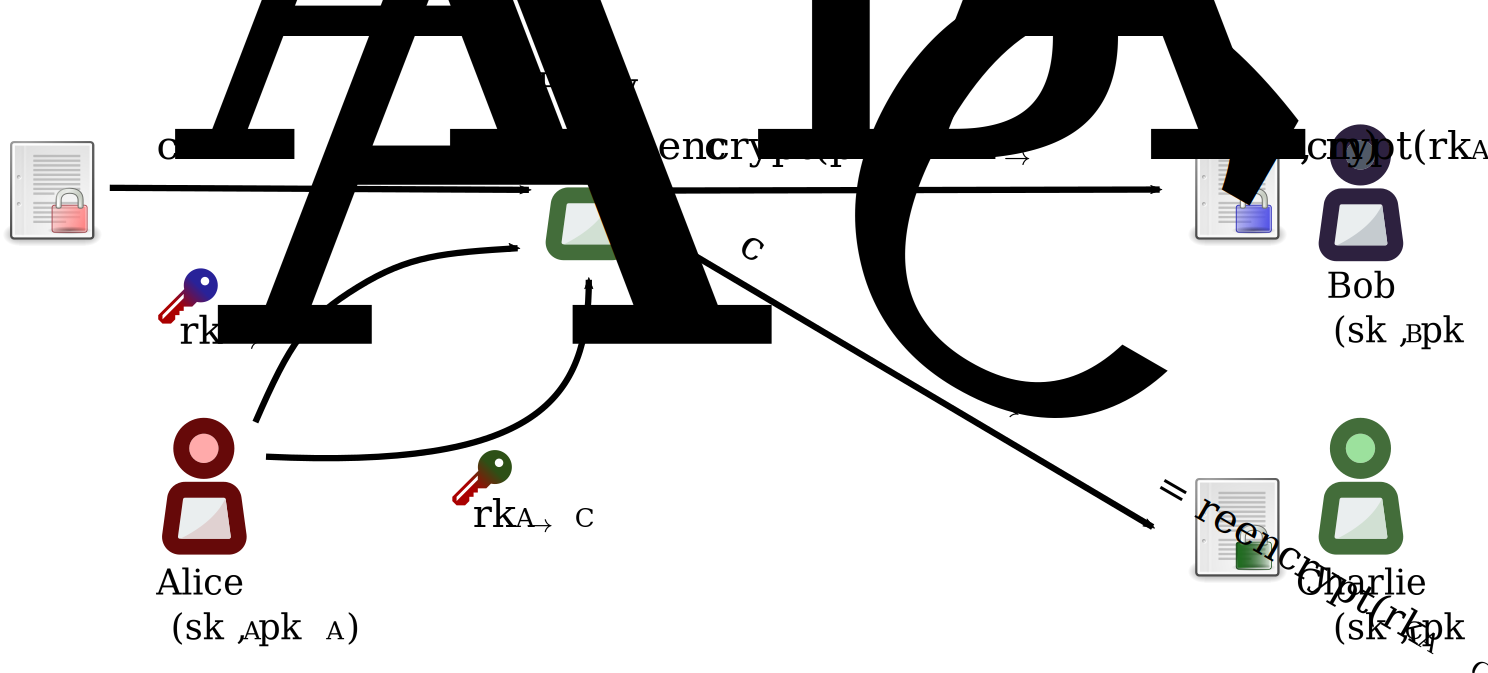
\includegraphics[width=13cm]{pdf/pre-multi.pdf}
        \end{figure}
        \href{run:videos/pre-explainer.mp4}{Proxy re-encryption video}
    \end{frame}

    \begin{frame}
        \frametitle{Solution}
        \framesubtitle{Proxy re-encryption + decentralization}
        \begin{figure}
            \centering
            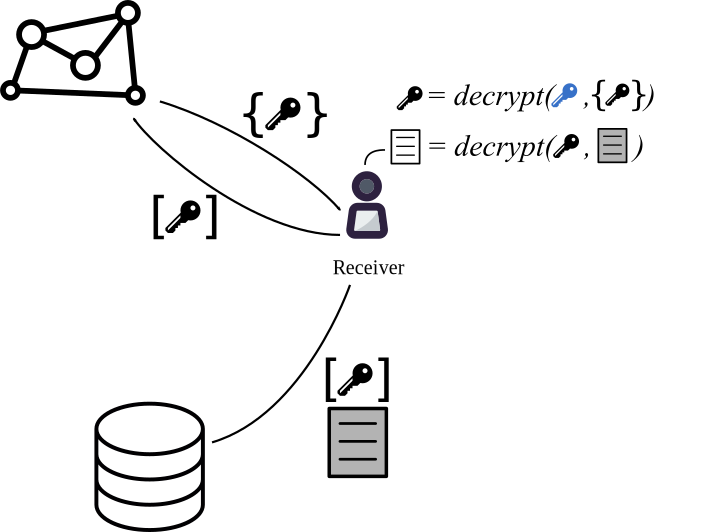
\includegraphics[height=6.5cm]{pdf/pre-kms.pdf}
        \end{figure}
    \end{frame}

    \begin{frame}
        \frametitle{Centralized KMS using PRE}
        \framesubtitle{Encryption}
        \begin{figure}
            \centering
            \includegraphics[height=7cm]{pdf/encrypt.pdf}
        \end{figure}
    \end{frame}

    \begin{frame}
        \frametitle{Centralized KMS using PRE}
        \framesubtitle{Access delegation}
        \begin{figure}
            \centering
            \includegraphics[height=7cm]{pdf/delegate.pdf}
        \end{figure}
    \end{frame}

    \begin{frame}
        \frametitle{Centralized KMS using PRE}
        \framesubtitle{Decryption}
        \begin{figure}
            \centering
            \includegraphics[height=7cm]{pdf/decrypt.pdf}
        \end{figure}
    \end{frame}

    \begin{frame}
        \frametitle{Decentralized Key Management}
        \framesubtitle{Using threshold split-key re-encryption (Umbral)}
        \begin{figure}
            \centering
            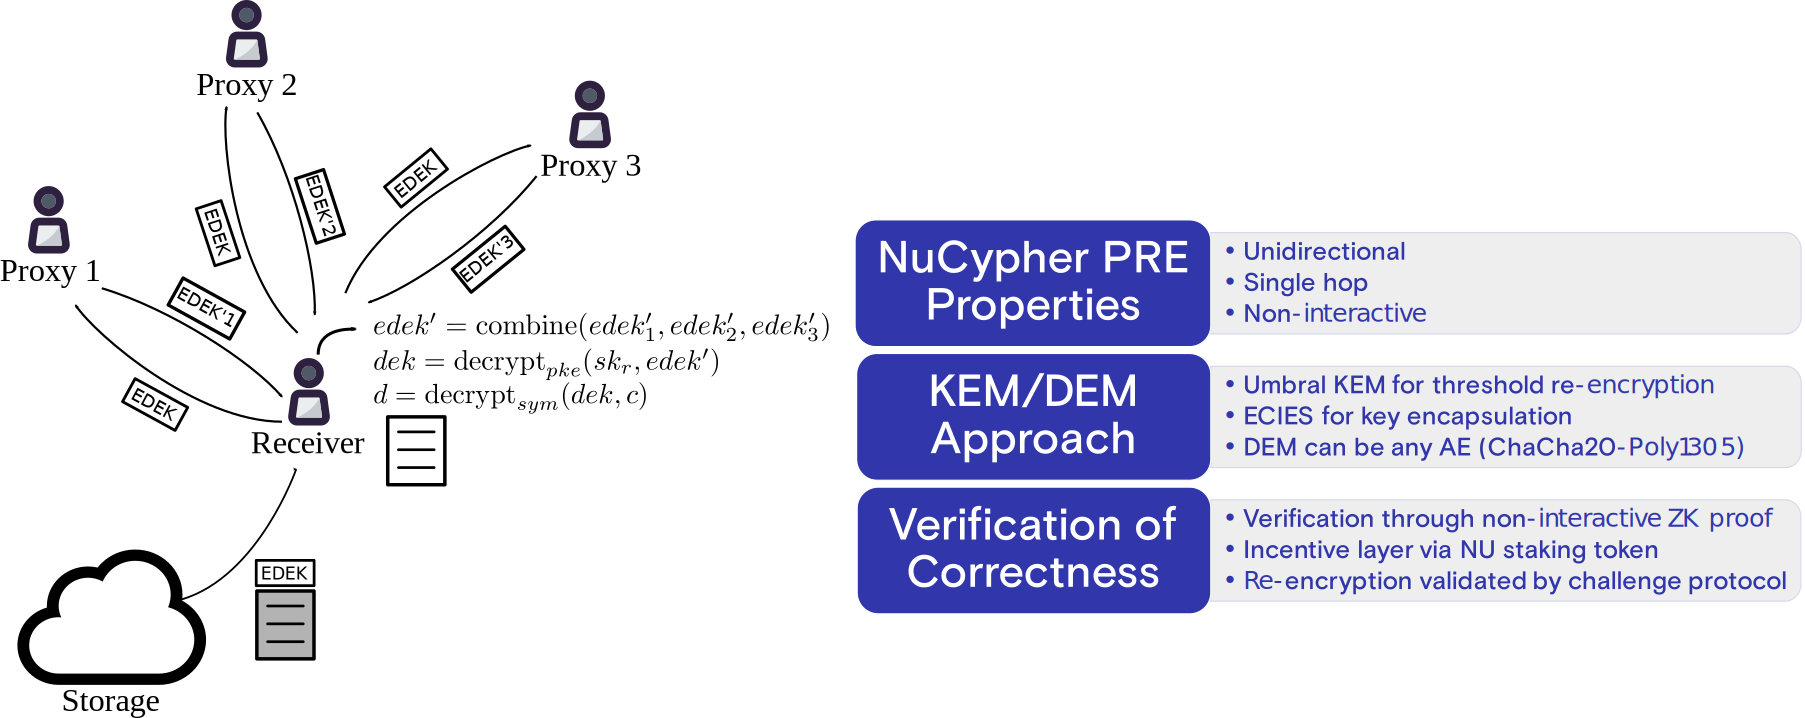
\includegraphics[height=6.5cm]{pdf/decrypt-umbral.pdf}
        \end{figure}
    \end{frame}

    \begin{frame}
        \frametitle{Umbral: Threshold Proxy Re-encryption}
        \begin{itemize}
        	\item \emph{``Umbral''} is Spanish for \emph{``threshold''}
            \item PRE properties: Unidirectional, single-hop, non-interactive
            \item Follows a KEM/DEM approach:
            	\begin{itemize}
		    \item UmbralKEM provides the threshold re-encryption capability
                    \item Uses ECIES for key encapsulation with ZK proofs of correctness for verifiability on prime order curves (such as secp256k1)
            	    \item DEM can be any authenticated encryption (currently ChaCha20-Poly1305)
        	\end{itemize}
	    \item IND-PRE-CCA security
            \item Key splitting is analogous to Shamir Secret Sharing
	    \item Verification of re-encryption correctness through Non-Interactive ZK Proofs
            \item Reference implementation: \url{https://github.com/nucypher/pyUmbral}
	    \item Documentation: \url{https://github.com/nucypher/umbral-doc}
        \end{itemize}
    \end{frame}

    \begin{frame}
        \frametitle{NU Token}
        \framesubtitle{Purpose}
        \begin{itemize}
            \item Splitting trust across re-encryption nodes
            \begin{itemize}
              \item More tokens = more trust, more work, and more compensation
            \end{itemize}
            \item Proof of Stake for minting new coins according to the mining schedule
            \item Security deposit at stake against malicious behavior of nodes
        \end{itemize}
    \end{frame}

    \begin{frame}[fragile]
        \frametitle{Where to start}
        \begin{verbatim}
virtualenv _venv -p python3
source _venv/bin/activate
pip3 install pip3 install git+https://github.com/nucypher/nucypher.git@federated

git clone https://github.com/nucypher/nucypher.git
cd nucypher
git checkout federated
cd examples/finnegans_wake_demo
python3 finnegans-wake-concise-demo.py
        \end{verbatim}
    \end{frame}

    \begin{frame}
        \frametitle{Demo with testnet}
        \begin{figure}
            \centering
            \includegraphics[height=5.5cm]{pdf/terminal.pdf}
        \end{figure}
        \href{run:videos/nucypher-node.mp4}{Extra: Video of testnet node running}
    \end{frame}

    \begin{frame}
      \frametitle{Early Users}
      \begin{figure}
           
\includegraphics[width=11.5cm]{pdf/projects.pdf}
      \end{figure}
    \end{frame}

    \begin{frame}
      \frametitle{Competing Technology}
       Data Masking and Tokenization
       \begin{itemize}
           \item Less secure for data with underlying patterns
           \item Reduce the value of data by obfuscating it
       \end{itemize}

       Public Key Encryption
       \begin{itemize}
           \item Data must be decrypted before it is shared
           \item Not Scalable
       \end{itemize}

       Multi-Party Computation
       \begin{itemize}
           \item Interactive protocol
           \item Slow Performance
       \end{itemize}

       Fully Homomorphic Encryption
       \begin{itemize}
           \item Slow Peformance
           \begin{itemize}
               \item NuCypher has developed a GPU-accelerated FHE library: nuFHE
           \end{itemize}
       \end{itemize}
     \end{frame}

    \begin{frame}
      \frametitle{Fully Homomorphic Encryption}
       \framesubtitle{nuFHE library}
       \begin{itemize}
           \item GitHub: \url{https://github.com/nucypher/nufhe}
           \item GPU implementation of fully homomorphic encryption
           \item Uses either FFT or integer NTT
           \item Achieved 100x performance over TFHE benchmarks
           \begin{figure}
               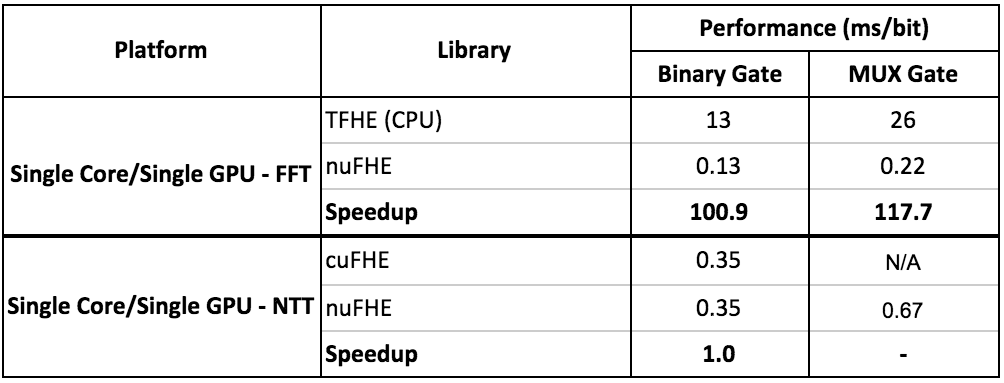
\includegraphics[width=10.5cm]{pdf/nufhe-benchmarks.pdf}
           \end{figure}
       \end{itemize}
     \end{frame}

    \begin{frame}
        \frametitle{API prize (2500 USD)}
        Anything of the following:
        \begin{itemize}
            \item Wrapper to interact with NuCypher network from Go, node.js,
                ...;
            \item Extension to interact with NuCypher network in browsers;
            \item Any exceptional dApp with good use of NuCypher for permission
                management.
        \end{itemize}
    \end{frame}

    \begin{frame}
        \frametitle{More Information}
        \begin{figure}
            \centering
            
\includegraphics[width=3cm]{pdf/nucypher_logo.pdf}
        \end{figure}
        Website: \url{https://www.nucypher.com}

        Whitepaper: \url{https://www.nucypher.com/whitepapers/english.pdf}

        Proxy Re-encryption Network: \url{https://github.com/nucypher/nucypher}

        Umbral Reference Implementation: \url{https://github.com/nucypher/pyUmbral}

        nuFHE: \url{https://github.com/nucypher/nufhe}

        Discord: \url{https://discord.gg/7rmXa3S}

        E-mail: \href{mailto:\emailname @nucypher.com}{\emailname @nucypher.com}

        E-mail: \href{mailto:hello@nucypher.com}{hello@nucypher.com}
    \end{frame}

    \begin{frame}
      \frametitle{Appendix: Umbral Flow Diagram}
      \begin{figure}
        \centering
        \includegraphics[width=11cm]{pdf/umbral-kem-flow.pdf}
      \end{figure}
      \begin{itemize}
           \item Reference implementation: \url{https://github.com/nucypher/pyUmbral}
           \item Documentation: \url{https://github.com/nucypher/umbral-doc}
      \end{itemize}
    \end{frame}

    \begin{frame}
        \frametitle{Appendix: Security Audits}
        \begin{figure}
            \centering
            
\includegraphics[height=2.5cm]{pdf/security-audits.pdf}
      \end{figure}
    \end{frame}

    \begin{frame}
        \frametitle{Appendix: NU Token Metrics}
        \framesubtitle{Mining}
        Mining \& Staking Economics: \url{https://github.com/nucypher/mining-paper}

        \bigskip

        Mining reward:
        \begin{align}
            \kappa &= \left(0.5 + 0.5\frac{\min(T_i, T_1)}{T_1}\right) \nonumber \\
            T_{i,\text{initial}} &\ge T_{\min} \nonumber \\
            \delta s_{i,t} &=  \kappa\, \frac{l_i}{\sum l_j} \frac{\ln{2}}{T_{1/2}} \left( S_{\max} - S_{t-1}\right) \nonumber
        \end{align}
        Results into:
        $$\text{reward} \propto 2^{\frac{t}{T_{1/2}}}$$
    \end{frame}

    \begin{frame}
        \frametitle{Appendix: NU Token Metrics}
        \framesubtitle{Graph of daily mining compensation}
        \begin{figure}
            \centering
            \includegraphics[height=5.5cm]{pdf/daily-compensation.pdf}
        \end{figure}
    \end{frame}

    \begin{frame}
        \frametitle{Appendix: NU Token Metrics}
        \framesubtitle{Relocking mining rewards}
        \begin{figure}
            \centering
            \includegraphics[height=5.5cm]{pdf/total-compensation.pdf}
        \end{figure}
    \end{frame}

    \begin{frame}
      \frametitle{Appendix: Team}
        \begin{figure}
            \centering
            \includegraphics[width=15cm]{pdf/company.pdf}
        \end{figure}
    \end{frame}

\end{document}

